



%%%%%%%%%%%%%%%%%%%%%%%%%%%%%%%%%%%%%%%%%%%%%%%%%%%%%%%%%%%%%%%%%%%%%%%%%%%%%
%%%%%%%%%%%%%%%%%%%%%%%%%%%%%%%%%%%%%%%%%%%%%%%%%%%%%%%%%%%%%%%%%%%%%%%%%%%%%
%%%%%%%%%%%%%%%%%%%%%%%%%%%%%%%%%%%%%%%%%%%%%%%%%%%%%%%%%%%%%%%%%%%%%%%%%%%%%
%%%%%%%%%%%%%%%%%%%%%%%%%%%%%%%%%%%%%%%%%%%%%%%%%%%%%%%%%%%%%%%%%%%%%%%%%%%%%
%%%%%%%%%%%%%%%%%%%%%%%%%%%%%%%%%%%%%%%%%%%%%%%%%%%%%%%%%%%%%%%%%%%%%%%%%%%%%
%%%%%%%%%%%%%%%%%%%%%%%%%%%%%%%%%%%%%%%%%%%%%%%%%%%%%%%%%%%%%%%%%%%%%%%%%%%%%
%%%%%%%%%%%%%%%%%%%%%%%%%%%%%%%%%%%%%%%%%%%%%%%%%%%%%%%%%%%%%%%%%%%%%%%%%%%%%
%%%%%%%%%%%%%%%%%%%%%%%%%%%%%%%%%%%%%%%%%%%%%%%%%%%%%%%%%%%%%%%%%%%%%%%%%%%%%
%%%%%%%%%%%%%%%%%%%%%%%%%%%%%%%%%%%%%%%%%%%%%%%%%%%%%%%%%%%%%%%%%%%%%%%%%%%%%
%%%%%%%%%%%%%%%%%%%%%%%%%%%%%%%%%%%%%%%%%%%%%%%%%%%%%%%%%%%%%%%%%%%%%%%%%%%%%






\begin{frame}
 \frametitle{Demo 2-1 $\vert$ \bfseries Thermostatics}
 \framesubtitle{\bfseries prescribed heat flux and heat source}
 \begin{overlayarea}{0.9\textwidth}{0.9\textheight}
%  \vspace*{1ex}
 \begin{center}
 \begin{tikzpicture}[scale=2]
  \onslide<1>{
  \fill[gray!10, draw=black] (0, 1) rectangle (3, 0) node[above left, black]{$\mathcal{B}$};
  }

    \onslide<1->{
  \fill[gray] (0.0, 0.0) rectangle (-0.05, 1.0);
%   \fill[pattern=north west lines, pattern color=black] (0, -0.25) rectangle +(-0.25, 1.5);
%   \draw[thick] (0, -0.25) -- +(0, 1.5);
%    \fill[pattern=north west lines, pattern color=black] (3, -0.25) rectangle +(0.25, 1.5);
%    \draw[thick] (3, -0.25) -- +(0, 1.5);
  }
  \onslide<1>{\draw (-0.05, 0.5) node[above, rotate=90] {$\theta^p=0^\circ\mathrm{C}$};}
  
  \onslide<1>{
  \draw[thin,gray] (0, 0) -- +(0, -0.5);
  \draw[thin,gray] (3, 0) -- +(0, -0.5);
  \draw[<->,thin,gray] (0, -0.4) -- node[fill=white]{$3 \ell$} +(3, 0);
  \draw[thin,gray] (3, 0) -- +(1.0, 0);
  \draw[thin,gray] (3, 1) -- +(1,0, -0);
  \draw[<->,gray] (3.9, 0) -- node[fill=white,sloped]{$\ell$} +(0, 1);

   \draw[thick,-latex] (0,0) -- +(0.5, 0) node[below]{$\v e_1$};
   \draw[thick,-latex] (0,0) -- +(0, 0.5) node[right]{$\v e_2$};
  }
  
  \onslide<1>{
  \foreach \y in {0.0, 0.25,0.5,...,1.0}
  \draw[decorate,decoration={snake, amplitude=1pt, segment length=5pt, post length=3pt},-latex] (3.5, 0.05+0.9/1.0*\y) -- +(-0.5, 0);  
%   \draw (0.05, 1.5) -- node[above]{$10 \,\mathrm{MPa}$} +(2.9, 0);
%   \draw (0.05, 1.5) -- +(2.9, 0);
  \node at (3.5, 1.0) [above,yshift=0.0cm]{$q^p$};
  \foreach \a in {0.0,45.0,90.0,...,315.0}
  \draw[decorate,decoration={snake, amplitude=1pt, segment length=5pt, post length=3pt},-latex,xshift=1cm, yshift=0.33cm] (\a:0.05cm) -- (\a:0.3cm);
  \node at (1.3, 0.5) {$r$};
  }

  \onslide<2>{
  \node at(1.5,0.5) {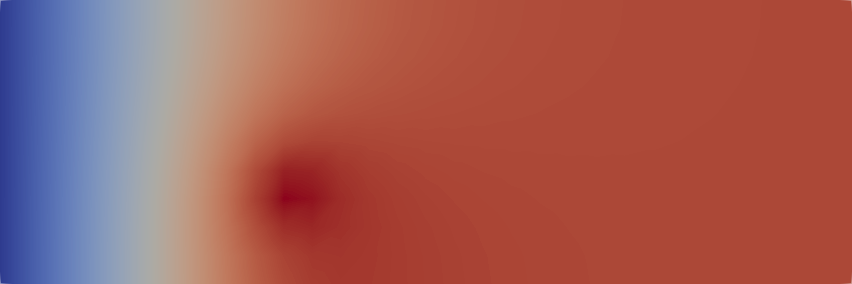
\includegraphics[width=6cm]{../02-thermo-static/01-heatsource/plot.png}};
  \begin{scope}[xshift=3.5cm,yshift=1.3cm,scale=0.5]
   \begin{axis}[thermobar,point meta min=0.0,point meta max=36.0,title={$\theta$ in $^\circ\mathrm{C}$}] 
    \addplot [draw=none] coordinates {(0,0)}; \end{axis}
  \end{scope}   
  }

  \end{tikzpicture}
  \end{center}
  
   \onslide<1>{
   \vspace*{-5ex}
   \begin{align*}
   \kappa &= 1 \, \tfrac{\mathrm{W}}{\mathrm{m} \cdot \mathrm{K}} & r &= 100 \,\exp \big(\tfrac{\vert \v x - \v x_0 \vert^2}{0.01 \, \ell^2} \big) \tfrac{\mathrm{MW}}{\mathrm{m}^3} \\
   \ell &= 0.1\,\mathrm{m} & q^p &= 1 \, \tfrac{\mathrm{W}}{\mathrm{m}^2}
   \end{align*}
   }

 \end{overlayarea}
\end{frame}



\begin{frame}
 \frametitle{Demo 2-2 $\vert$ \bfseries Thermostatics}
 \framesubtitle{\bfseries non-homogeneous heat conduction coefficient}
 \begin{overlayarea}{0.9\textwidth}{0.9\textheight}
%   \vspace*{-1cm}
 \begin{center}
 \begin{tikzpicture}[scale=2]
  \onslide<1>{
  \fill[gray!10, draw=black] (0, 1) rectangle (3, 0) node[above left, black]{$\mathcal{B}$};
  }

    \onslide<1->{
  \fill[gray] (0.0, 0.0) rectangle +(-0.05, 1.0);
  \fill[gray] (3.0, 0.0) rectangle +(0.05, 1.0);
%   \fill[pattern=north west lines, pattern color=black] (0, -0.25) rectangle +(-0.25, 1.5);
%   \draw[thick] (0, -0.25) -- +(0, 1.5);
%    \fill[pattern=north west lines, pattern color=black] (3, -0.25) rectangle +(0.25, 1.5);
%    \draw[thick] (3, -0.25) -- +(0, 1.5);
  }
  \onslide<1>{
  \draw (-0.05, 0.5) node[above, rotate=90] {$\theta^p=25^\circ\mathrm{C}$};
  \draw (3.05, 0.5) node[below, rotate=90] {$\theta^p=-10^\circ\mathrm{C}$};
  
  \node at (0.5, 0.5) {$\kappa_1$};
  \node at (1.5, 0.5) {$\kappa_2$};
  \node at (2.5, 0.5) {$\kappa_3$};
 }
  
  \onslide<1>{
  \foreach \x in {0.0, 1.0, 2.0} {
    \draw[thin,gray] (\x, 0) -- +(0, -0.5);
    \draw[<->,thin,gray] (\x, -0.4) -- node[fill=white]{$\ell$} +(1, 0);
   };
  \draw[thin,gray] (3, 0) -- +(0, -0.5);
  
  \draw[thin,gray] (3, 0) -- +(1.0, 0);
  \draw[thin,gray] (3, 1) -- +(1.0, -0);
  \draw[<->,gray] (3.9, 0) -- node[fill=white,sloped]{$\ell$} +(0, 1);

   \draw[thick,-latex] (0,0) -- +(0.5, 0) node[below]{$\v e_1$};
   \draw[thick,-latex] (0,0) -- +(0, 0.5) node[right,xshift=-0.1cm]{$\v e_2$};
  }
  
%   \onslide<1>{
%   \foreach \y in {0.0, 0.25,0.5,...,1.0}
%   \draw[decorate,decoration={snake, amplitude=1pt, segment length=5pt, post length=3pt},-latex] (3.5, 0.05+0.9/1.0*\y) -- +(-0.5, 0);  
% %   \draw (0.05, 1.5) -- node[above]{$10 \,\mathrm{MPa}$} +(2.9, 0);
% %   \draw (0.05, 1.5) -- +(2.9, 0);
%   \node at (3.5, 1.0) [above,yshift=0.0cm]{$q^p$};
%   \foreach \a in {0.0,45.0,90.0,...,315.0}
%   \draw[decorate,decoration={snake, amplitude=1pt, segment length=5pt, post length=3pt},-latex,xshift=1cm, yshift=0.33cm] (\a:0.05cm) -- (\a:0.3cm);
%   \node at (1.3, 0.5) {$r$};
%   }

  \onslide<2>{
  \node at(1.5,0.5) {
\includegraphics[width=6cm]{../02-thermo-static/02-wall/plot.png}};
  \begin{scope}[xshift=3.5cm,yshift=1.3cm,scale=0.5]
   \begin{axis}[thermobar,point meta min=-10.0,point meta max=25.0,title={$\theta$ in $^\circ\mathrm{C}$}] 
    \addplot [draw=none] coordinates {(0,0)}; \end{axis}
  \end{scope}   
  }
  
  \onslide<1->{
  \draw[dashed] (1.0, 0.0) -- +(0.0, 1.0);
  \draw[dashed] (2.0, 0.0) -- +(0.0, 1.0);
  }

  \end{tikzpicture}
  \end{center}
   
   \vspace*{-0.5cm}
   \only<1>{
   \begin{align*}
   \kappa_1 &= 2.0 \, \tfrac{\mathrm{W}}{\mathrm{m} \cdot \mathrm{K}} &&\text{(concrete)}\\
   \kappa_2 &= 0.3 \, \tfrac{\mathrm{W}}{\mathrm{m} \cdot \mathrm{K}} &&\text{(PU foam)}\\
   \kappa_3 &= 1.0 \, \tfrac{\mathrm{W}}{\mathrm{m} \cdot \mathrm{K}} &&\text{(brick)}\\
   \end{align*}
   }
%    \\
   \only<2>{
   \hspace*{0.2cm}
   \begin{tikzpicture}
    \node at(1.5,0.5) {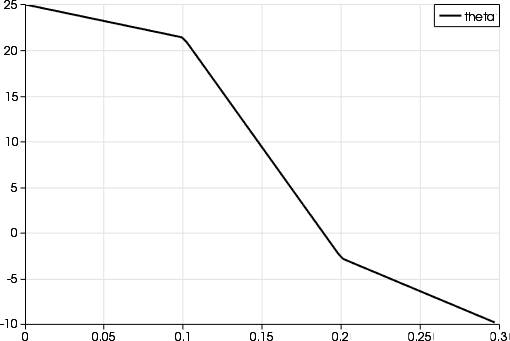
\includegraphics[width=6.4cm,height=3cm]{../02-thermo-static/02-wall/plot_linear.png}};
   \end{tikzpicture}
   }
 \end{overlayarea}

\end{frame}




